\documentclass[10 pt, twocolumn]{article}

\usepackage[utf8]{inputenc}
\usepackage[T1]{fontenc}
\usepackage{caption}
\usepackage{graphicx}
\usepackage{xcolor}
\usepackage{interval}
\usepackage{listingsutf8}
\usepackage{hyperref}
\usepackage{siunitx}
\usepackage{algorithm2e}
\usepackage{rotating}
\usepackage{adjustbox}
\usepackage{booktabs}
\usepackage{pgfplots}
\usepackage{tikz}
\usepackage{footmisc}
\usepackage{amsfonts}
\usepackage[backend=biber,style=numeric]{biblatex}
\usepackage[
  left=1.50cm,
  right=1.50cm,
  top=2.00cm,
  bottom=2.00cm
]{geometry}

\pgfplotsset{compat=1.15}

\sisetup{load-configurations=abbreviations, binary-units=true}
\intervalconfig {
    soft open fences ,
    separator symbol =; ,
}

\lstdefinelanguage{JavaScript}{
  keywords={break, case, catch, continue, debugger, default, delete, do, else, finally, for, function, if, in, instanceof, new, return, switch, this, throw, try, typeof, var, void, while, with},
  morecomment=[l]{//},
  morecomment=[s]{/*}{*/},
  morestring=[b]',
  morestring=[b]",
  sensitive=true
}

\lstdefinelanguage{Protobuf}{
  keywords={message, string, uint32, int32},
  morecomment=[l]{//},
  morecomment=[s]{/*}{*/},
  morestring=[b]',
  morestring=[b]",
  sensitive=true
}

\lstset{
    language=C,
    keywordstyle={\bfseries},
    basicstyle=\footnotesize,
    literate={->}{$\rightarrow{}$}{1} {<-}{$\leftarrow{}$}{1},
    stringstyle=\color{purple},
    keepspaces=true,
    captionpos=b,
    inputencoding=utf8,
    escapeinside={\%*}{*)}
}

\renewcommand\AlCapSty{\text}
\SetAlCapNameFnt{\footnotesize}
\SetAlCapFnt{\footnotesize}
\SetAlgoCaptionSeparator{.}
\DeclareCaptionLabelFormat{nospace}{#1 #2}
\captionsetup[table]{labelformat=nospace,labelfont=rm,name=Table,labelsep=period}

\newcommand{\pcode}[1]{
    \lstinline[basicstyle=\itshape,keywordstyle={}]{#1}
}

\newcommand*{\lstnumberautorefname}{line}

\newcommand{\icode}[1]{\lstinline{#1}}

\newcommand{\name}[1] {\emph{#1}}

\newcolumntype{R}[2]{%
    >{\adjustbox{angle=#1,lap=\width-(#2/2)}\bgroup}%
    l%
    <{\egroup}%
}
\newcommand*\rot{\multicolumn{1}{R{90}{1em}}}

\newcommand{\fig}[3]{
  \begin{figure}[h]
    \begin{center}
        \includegraphics[width=8cm,keepaspectratio]{#1}
        \caption{#3}
        \label{fig:#2}
    \end{center}
  \end{figure}
}

\usepackage[most]{tcolorbox}
\newcounter{example}
\usepackage{xparse}
\usepackage{lipsum}

\def\exampletext{Example} % If English
\NewDocumentEnvironment{example}{ O{} }
{
\colorlet{colexam}{red!55!black} % Global example color
\newtcolorbox[use counter=example]{examplebox}{%
    % Example Frame Start
    empty,% Empty previously set parameters
    title={#1},% use \thetcbcounter to access the example counter text
    % Attaching a box requires an overlay
    attach boxed title to top left,
       % Ensures proper line breaking in longer titles
       minipage boxed title,
    % (boxed title style requires an overlay)
    boxed title style={empty,size=minimal,toprule=0pt,top=4pt,left=3mm,overlay={}},
    coltitle=colexam,fonttitle=\bfseries,
    before=\par\medskip\noindent,parbox=false,boxsep=0pt,left=3mm,right=0mm,top=2pt,breakable,pad at break=0mm,
       before upper=\csname @totalleftmargin\endcsname0pt, % Use instead of parbox=true. This ensures parskip is inherited by box.
    % Handles box when it exists on one page only
    overlay unbroken={\draw[colexam,line width=.5pt] ([xshift=-0pt]title.north west) -- ([xshift=-0pt]frame.south west); },
    % Handles multipage box: first page
    overlay first={\draw[colexam,line width=.5pt] ([xshift=-0pt]title.north west) -- ([xshift=-0pt]frame.south west); },
    % Handles multipage box: middle page
    overlay middle={\draw[colexam,line width=.5pt] ([xshift=-0pt]frame.north west) -- ([xshift=-0pt]frame.south west); },
    % Handles multipage box: last page
    overlay last={\draw[colexam,line width=.5pt] ([xshift=-0pt]frame.north west) -- ([xshift=-0pt]frame.south west); },%
    }
\begin{examplebox}}
{\end{examplebox}\endlist}

\newcommand*\circled[1]{\tikz[baseline=(char.base)]{
            \node[shape=circle,draw,inner sep=1pt] (char) {#1};}}

\usepackage{tikz}

\newcommand{\smiley}{\tikz[baseline=-0.75ex,black]{
    \draw circle (2mm);
\node[fill,circle,inner sep=0.5pt] (left eye) at (135:0.8mm) {};
\node[fill,circle,inner sep=0.5pt] (right eye) at (45:0.8mm) {};
\draw (-145:0.9mm) arc (-120:-60:1.5mm);
    }
}

\newcommand{\frownie}{\tikz[baseline=-0.75ex,black]{
    \draw circle (2mm);
\node[fill,circle,inner sep=0.5pt] (left eye) at (135:0.8mm) {};
\node[fill,circle,inner sep=0.5pt] (right eye) at (45:0.8mm) {};
\draw (-145:0.9mm) arc (120:60:1.5mm);
    }
}

\newcommand{\neutranie}{\tikz[baseline=-0.75ex,black]{
    \draw circle (2mm);
\node[fill,circle,inner sep=0.5pt] (left eye) at (135:0.8mm) {};
\node[fill,circle,inner sep=0.5pt] (right eye) at (45:0.8mm) {};
\draw (-135:0.9mm) -- (-45:0.9mm);
    }
}


\addbibresource{root.bib}

\title{Protocol chaos}

\author{Jan Macháček, Miguel Lopez, Matthew Squire}

\begin{document}

\twocolumn[
  \begin{@twocolumnfalse}
    \maketitle
    \begin{abstract}
      Chaos engineering is a way to introduce unexpected failures in order to discover a system's failure modes. The chaos engineering tools usually introduce faults that focus on the connections between the system's components by disrupting the expected operation of the network (by introducing latency, packet loss, all the way to complete network partitions) or by disrupting the operation of the nodes hosting the components (by reducing the available CPU or memory resources). Our work on chaos testing showed that this is not only insufficient, but that more ``damage'' can be achieved by focusing first on how a system handles unexpected input--trivially structurally invalid messages; or structurally valid messages that contain invalid values; or strucurally valid messages with valid, yet damaging or malicious values. Once the system can reliably handle invalid and malicious inputs, the infrastructure chaos engineering can be used to tease out further failure scenarios. 
    \end{abstract}
  \end{@twocolumnfalse}
]

\section{Protocol chaos}
Validation of inputs is acklowledged to be important, yet it is very often not implemented as thoroughly as it should be; not for the lack of understanding its importance, but for the effort it requires. Consider a component that accepts a message to announce a greeting $n$ numer of times; it exposes a REST endpoint at \pcode{POST /greeting} and expects a message with the \pcode{greeting} and \pcode{count} values. The description of the service and the field names in the input message provide intuition about the expected values: the \pcode{greeting} can be one of \pcode{\{ "hello", "hi", "top of the afternoon to you, sir!"\}} and similar; the value for \pcode{count} is an integer in the range of $\interval[open]{1}{5}$. The first level of validation is to check that the values posted indeed represent valid ``types'' (the \pcode{greeting} is text; the \pcode{count} is an integer). This is "included for free" in strongly-typed languages if the input message uses appropriate types for its members; and it is simple to do in weakly-typed languages. The next level of validation should focus on acceptable range of values. For the \pcode{count} property, the validation code should verify that it is indeed in the range of (say) $\interval[open]{1}{5}$. The validation code for the \pcode{greeting} property can be more complex: it is difficult to precisely define valid or invalid \pcode{string}. The possible invalid examples include empty string, very long string, etc; though it remains easy to find an invalid string that nevertheless passes the validation code, and it is just as easy to find valid string that fails. (Consider "Good morning, Llanfairpwllgwyngyllgogerychwyrndrobwllllantysiliogogogoch!": it is perfectly valid greeting in a small village in North Wales.) If discovering the validation rules for \pcode{greeting} is difficult, it is even more difficult to exhaustively test those rules. 

It is possible to implement a test that verifies that the system under test processes the message as expected. However, this is a very broad requirement, so it is usually split into multiple \emph{unit} tests. But even with this split, the initial problem of imagining and then coding the possible messages still remains. In order to allow valid messages conforming to some protocol to be generated, there needs to be a machine-readable description of the protocol. This description needs to include the elements and their types. The types should include at least integer numbers, floating point numbers, strings, enumerations, arrays, maps, and other messages; it is useful if the protocol description can describe sum types. The protocol tooling should also be able to take the protocol descriptions and generate source code for the target language and framework combination. Protocol Buffers \cite{protobuf} is an example of the protocol definition language and rich tooling that satisfies these requirements. The code in \autoref{code:pb-example} shows how to define a message \pcode{X} with two fields in the Protocol Buffers syntax.

\begin{lstlisting}[caption={Trivial protocol definition}, label={code:pb-example}, language=Protobuf]
message X {
    int32 count = 1;
    string greeting = 2; 
}
\end{lstlisting}

Given this definition, the Protocol Buffers tooling can be used to generate the source code for Scala, Swift, C++, and many other languages. The generated code for each message includes definition of the protocol; the definition is shown in pseudo-code in \autoref{code:pb-definition-pseudo}.

\begin{lstlisting}[caption={Trivial protocol definition}, label={code:pb-definition-pseudo}, language=JavaScript, escapechar=|]
|The message $X$ contains two fields, both optional.|
name: "X"
|$count$, of type \SI{32}{\bit} signed integer|
field {
  name: "count"
  number: 1
  label: LABEL_OPTIONAL
  type: TYPE_INT32
  json_name: "count"
}
|$greeting$, of type UTF-8 string|
field {
  name: "greeting"
  number: 2
  label: LABEL_OPTIONAL
  type: TYPE_STRING
  json_name: "greeting"
}
\end{lstlisting}

Using this definition, it is possible to devise a generator that examines the types of the fields, and emits possible values that conform to the field's type: the range of values for \pcode{int32} includes $\{0, 1, 64, 2^{31}-1, -2^{31}+1, -100, -1\}$; the range of values for \pcode{string} includes empty, short alphanumeric, long alphanumeric, and even more values can be found on The Big List of Naughty Strings \cite{blns}. Generators for other types follow similar pattern in the samples they provide. It is useful to add heuristics to the generator, making it consider the field name in addition to the field type. This way, a generator for field \pcode{url} can generate (malicious) URLs in addition to simply one of the \emph{naughty strings}. The range of values that the generator can emit for each type is very large, the generator needs to take--in addition to the field definition--a random number generator and emits a structure that can be used to combine with other generators. See \autoref{code:pb-generator} for an example in ScalaCheck.

\begin{lstlisting}[caption={Generator}, label={code:pb-generator}, language=Scala, escapechar=|]
object MessageGenerator {
  |Constructs a generator for a type of type $A$, with optionally|
  |provided hints for the fields|
  def msg[A <: GeneratedMessage with Message[A]]
      (implicit cmp: GeneratedMessageCompanion[A], 
       hint: Hint[A] = noHint): Gen[A] = ...

  |The default hints that can be imported into scope where|
  |$msg$ is used|
  object hints {
    implicit def default[A]: Hint[A] = ...
  }

  |Hint for type $A$ is able to provide specific generator for the given $fd$|
  trait Hint[+A] {
    def hint(fd: FieldDescriptor): Option[Gen[Any]]
  }

}

|To use it, we prepare the parameters and seed for the application of the generators|
val parameters = Gen.Parameters
                  .default
                  .withSize(1999)
def seed = Seed(System.currentTimeMillis())
import MessageGenerator._
import hints._

|Generate one "chaotic" instance of message $X$, using the in-scope $Hints[X]$|
val x = msg[X](parameters, seed)
println(x)
\end{lstlisting}

Several executions of the code above yielded usefully-damaged instances of message $X$ (shown in \autoref{code:pb-generator-applied}); these instances were indeed valid according to the protocol definition, but some of the values can be considered unusual. 

\begin{lstlisting}[caption={Generator examples}, label={code:pb-generator-applied}, language=Scala, escapechar=|]
X(count: -4959664 greeting: "dlnz6hbbfeb6ofu...")
X(count: 0 greeting: "dlnz6hbbfeb6ofu...")
X(count: -1 greeting: "dlnz6hbbfeb6ofu...")
X(count: 1 greeting: "dlnz6hbbfeb6ofu...")
...
X(count: 0 greeting: "sqjsY8y3bvhg3az...")
\end{lstlisting}

Even though this code is specific to ScalaCheck\cite{scalacheck} in Scala, there are similar \emph{property-based} testing frameworks available for other languages (such as RapidCheck\cite{rapidcheck} for C++, SwiftCheck\cite{swiftcheck} for Swift, and similar). 

\section{Security and integrity}
It is important to consider the attack vectors on the protocol (how easy is it to construct a malicious message) that causes unexpected behavior in the protocol implementations; it is just as important to understand the resilience of the protocol's wire format against transmission errors. This should inform the design of security and integrity measures, which can range from simple CRC checksums to cryptographic signatures and encryption\footnote{Doing nothing is dangerous, particularly for systems that are exposed to other systems or even the Internet.}. 

\subsection{Integrity}
Message integrity mechanisms detect errors in the layers that follow the construction of the message. These layers include not only the network transport, but also the protocol codecs, networking libraries, etc. For example, Kafka\cite{apache-kafka} defines maximum message size. The wire format plays an important role in being able to detect failures in the messages' integrity. The proportion of useful data to the protocol wire format control structures defines the probability of a bit error damaging the message so that it cannot be decoded. Take the message in \autoref{code:trivial-protocol-definition}, which shows a message in the Protocol Buffer language.

\begin{lstlisting}[caption={Trivial protocol definition}, label={code:trivial-protocol-definition}, language=Protobuf]
message X {
    int32 count = 1;
    string greeting = 2; 
}
\end{lstlisting}

A wire format of a message conforming to this protocol with \pcode{count -> 42; greeting -> "Hello, world"} is shown in \autoref{fig:wire-format-density-json} and \autoref{fig:wire-format-density-pb}.

\fig{wire-format-density-json.png}{wire-format-density-json}{JSON wire representation}

\fig{wire-format-density-pb.png}{wire-format-density-pb}{Protocol Buffers binary wire representation}

The binary representation directly maps to the bytes that make up the \SI{4}{\byte} \pcode{int32} value and the \pcode{string} with length \pcode{0x0c}. There are only \SI{3}{\byte} that appear on the wire in addition to the useful information. The JSON representation contains \SI{28}{\byte} that are included on the wire in addition to the useful information; moreover, the value \pcode{42} has to be translated from a textual representation to the \pcode{int32} value. Consider a situation of a bit error on the wire in 1 random byte. The probability of hitting the bytes that form the wire format is $3/16$ in the Protocol Buffers wire format; and $7/4$ in the JSON wire format. The damage to the message is therefore more likely to be detectable by parsing errors in the less dense JSON representation (see \autoref{fig:wire-format-density-err}).

\fig{wire-format-density-err.png}{wire-format-density-err}{Bit error impact}

The more dense the wire representation is, the more important it is to include bit error detection. A simple checksum using CRC32 \cite{crc32} is sufficient for systems with low to moderate message rates. A parallel (though CPU-bound) implementation of \autoref{alg:bit-damage}, capable of brute-forcing \SI{1200000}{messages \per \second} per second on i7-7920HQ CPU took \SI{1564.6}{\second} (averaged over 10 runs) to find one instance of conflicting message\footnote{Even though it is easy to find \emph{different} messages that have the same CRC32 value, it is difficult to find messages that share the same CRC32 value, but differ only by a few bits \emph{and} are valid wire format representations.}.

\begin{algorithm}
  \caption{Bit damage}
  \label{alg:bit-damage}
  \DontPrintSemicolon
  \KwData{generator $g$ of instances of $X$ with sufficiently large number of bits}
  \KwResult{message $x$, its wire representation $b$ and damaged wire representation $b'$ such that $b'$ is valid according to the protocol format: $b \neq b' \land deser(b) \neq deser(b') \land checksum(b) = checksum(b')$}
  \While{true}{
    $x \leftarrow g()$\;
    $b \leftarrow ser(x)$\;
    $c \leftarrow checksum(b)$\;
    \Repeat{$damaged\mbox{-}bits(b') < threshold$} {
      $b' \leftarrow damage(b)$\;
      $c' \leftarrow checksum(b')$\;
      \If{$c = c' \land deser(b) \neq deser(b')$} {
        \Return{$x, b, b'$}
      }
    }
  }
\end{algorithm} 

An example of such conflicting message of type \pcode{X} from \autoref{code:trivial-protocol-definition} is shown in \autoref{tbl:bit-damage}. The messages have the same \pcode{count} property (set to 583145568), differ in the \pcode{greeting} property by \SI{19}{\bit}s, yet share the same CRC32 value (1540204925). Consider a system that includes a component that "reliably" introduces random bit errors and handles \SI{120000}{messages \per \second}. The interval between undetectable damage to messages that rely on CRC32 to detect errors will be only \SI{4}{\hour}!

\begin{table}[h]
    \begin{tabular}{r*{9}{l}}
        \toprule
        $idx$ & \rot{492} & \rot{493} & \rot{521} & \rot{680} 
        & \rot{689} & \rot{1052} & \rot{1760} 
        & \rot{2203} & \rot{2544} \\
        \midrule
        $greeting[idx]$  & U & ] & E                & ? & z & \textbar         &    & \% & v \\
        $greeting'[idx]$ & E & L & \textbackslash01 & * & 2 & \textbackslash32 & D  & !  & p \\
        \bottomrule
    \end{tabular}
    \caption{Bit damage}
    \label{tbl:bit-damage}
\end{table}

In a system that processes large number of messages, or if the possibility of encountering undetectable damaged messages is unacceptable (say in systems that deal with sensitive personal or financial information) use cryptographic hashes to verify the integrity of the messages. Unfortunately, this comes with computational overhead which is summarized in \autoref{tbl:integrity-overhead} (with CRC32 on \SI{1}{\kibi\byte} as the baseline).

\begin{table}[h]
\begin{minipage}{\hsize}
    \begin{tabular}{r*{6}{r}} % {rccccc}
        \toprule
        & \multicolumn{5}{c}{Message size} \\
        \cmidrule(r){2-6}
        Algorithm & \SI{100}{\byte} & \SI{1}{\kibi\byte} & \SI{10}{\kibi\byte} & \SI{100}{\kibi\byte} & \SI{1}{\mebi\byte} \\
        \midrule
        CRC32                                                                 &  3  &   1 &   7 &   606 &   9574 \\
        SHA-256\footnote{\label{shai}Intel SHA\cite{intel-sha256} extensions} &  9  &  26 & 118 & 11860 & 120595 \\
        SHA-256\footnote{\label{plain}Plain x86\_64 implementation}           & 50  & 150 & 681 & 68787 & 699450 \\ 
        SHA-512\footref{plain}                                                & 94  & 156 & 475 & 48619 & 487513 \\
        % MD5                                                                 & 125 & 50  & 344 & 31750 & 319631 \\
        \bottomrule
    \end{tabular}
    \caption{Integrity overhead}
    \label{tbl:integrity-overhead}
\end{minipage}
\end{table}

The results show that using robust cryptographic digest (SHA-256 or SHA-512) add significant overhead when compared to the simple CRC32 checksum, though on CPUs with the SHA extensions and matching implementation\footnote{For example, on x86\_64 CPUs it will be necessary to verify that the compiler / runtime emits the \pcode{SHA256RNDS2, SHA256MSG1, SHA256MSG2} instructions} the cost of the overhead is significantly lower.

JWT \cite{jwt} provides value semantics for authorisation, but also provides mechanisms to verify the integrity of the messages. JWT combines the message itself (called payload in JWT) and \emph{claims} that can be used for authorisation. 

% adds significant overhead: the producer has to compute the signature and the receiver has to verify it. Moreover, this adds the need to maintain secure key stores, which further complicates the system's infrastructure.

\subsection{Malicious messages}
A system can be attacked by sending it malicious input, aiming to either make it unavailable, or to make it perform operation that the attacker is not privileged to do. 

The denial-of-service style attacks aim to completely crash the nodes running the services; for example by causing out-of-memory or stack-overflow errors that the system should not catch, or causing high CPU usage, or by making the system under attack read too much data from an I/O device. An example of a message that causes stack-overflow exception in Protocol Buffers using \pcode{"com.google.protobuf" \% "protobuf-java" \% "3.4.0"} and \pcode{"com.trueaccord.scalapb" \%\% "compilerplugin" \% "0.6.6"}\cite{scalapb} is shown in \autoref{code:malicious-message-pb}.

\begin{lstlisting}[caption={Malicious message}, label={code:malicious-message-pb}, language=Scala, escapechar=|]
|Construct a malicious message that starts with the valid serialized bytes $b$ and adds 6000 bytes with the value 99.|
val b  = Array[Byte](8, 1, 18, 3)
val mb = Array.fill(6000)(99.toByte)
Array.copy(b, 0, mb, 0, b.length)

|Decode an instance of $X$ the input $mb$|
X.validate(mb) |\label{line:malicious-message-pb-so}|
|$\uparrow$|
|Exception in thread "main" java.lang.StackOverflowError|
|  at \ldots\$StreamDecoder.readTag(\ldots:2051)|
|  at \ldots\$StreamDecoder.skipMessage(\ldots:2158)|
|  at \ldots\$StreamDecoder.skipField(\ldots:2090)|
|  \ldots|
\end{lstlisting}

Other wire formats are just as susceptible to this type of attacks: sending too-deeply nested JSON causes the same behaviour in eager JSON parsers, for example \pcode{"org.json4s" \%\% "jackson" \% "3.5.1"} (viz \autoref{code:malicious-message-json}).

\begin{lstlisting}[caption={Malicious message}, label={code:malicious-message-json}, language=Scala, escapechar=|]
|Construct malicious JSON document|
val mj = """{"x":""" * 2000

|Decode an instance of $X$ from the input $mj$|
JsonFormat.fromJsonString[X](mj)
|$\uparrow$|
|Exception in thread "main" java.lang.StackOverflowError|
|  at \ldots JsonStreamContext.\textless{}init\textgreater(\ldots:43)|
|  at \ldots JsonReadContext.\textless{}init\textgreater(\ldots:58)|
|  at \ldots JsonReadContext.createChildObjectContext(\ldots:128)|
|  at \ldots ReaderBasedJsonParser.\_nextAfterName(\ldots:773)|
|  at \ldots ReaderBasedJsonParser.nextToken(\ldots:636)|
|  at \ldots JValueDeserializer.deserialize(\ldots:45)|
|  \ldots|
\end{lstlisting}

There is no way to catch the \pcode{StackOverflowError} arising from \pcode{JsonFormat.fromJsonString[X](mj)} and \pcode{X.validate(mb)} and the thread that attempted the decoding ends. This attack can be mitigated by moving the decoding to a thread; a suitable language \& framework makes this a fairly easy task. An example of safe, though very inelegant (because of the use of $Await.result$) code in Scala is shown in \autoref{code:so-mitigation}. The $decode$ function can be used as a direct replacement in your code (though production implementation should pay extra attention to properly configure the $ExecutionContext$ with sufficient number of threads and pinning behavior). Non-blocking toolkits (such as Akka\cite{akka} and Play\cite{play} in Scala) use non-blocking style throughout, which means that there is no need to block for the result of the asynchronous operation; the code in \autoref{code:so-mitigation} and the performance measurements represent the worst-case scenarios.

\begin{lstlisting}[caption={Stack Overflow Mitigation}, label={code:so-mitigation}, language=Scala, escapechar=|]
|The decoding function takes the bytes $b$ to decode and schedules the decoding in the $ec$. It returns the result of the decoding, but will survive a $StackOverflowError$.|
def decode(b: Array[Byte])
  (implicit ex: ExecutionContext): Try[X] = {
  import scala.concurrent.duration._
  val timeout = 100.milliseconds
  Try(Await.result(Future(X.parseFrom(b)), to))
}

|Construct "good" payload|
val b  = Array[Byte](8, 1, 12, 3, 65, 66, 67)
|Construct malicious payload|
val mb = Array[Byte](8, 1, 12, 3, 65, 66, 67, 
                     99, ..., 99)

|With an implicit $ExecutionContext$ in scope, applying $decode$ to the good payload $b$ returns $Success(X(...))$ in roughly \SI{17}{\milli \second}.|
decode(b)

|With an implicit $ExecutionContext$ in scope, applying $decode$ to the good payload $b$ returns $Failure(TimeoutException)$ after the timeout of \SI{100}{\milli \second} elapses.|
decode(mb)
\end{lstlisting}

While the code to implement the mitigation against this type of attack is straightforward, moving the decoding to another thread adds significant dispatch overhead (roughly 17 times the raw) to the decoding (see \autoref{plot:mitigation-overhead}). 

\begin{figure}[h]
  \caption{Mitigation overhead}
  \label{plot:mitigation-overhead}
  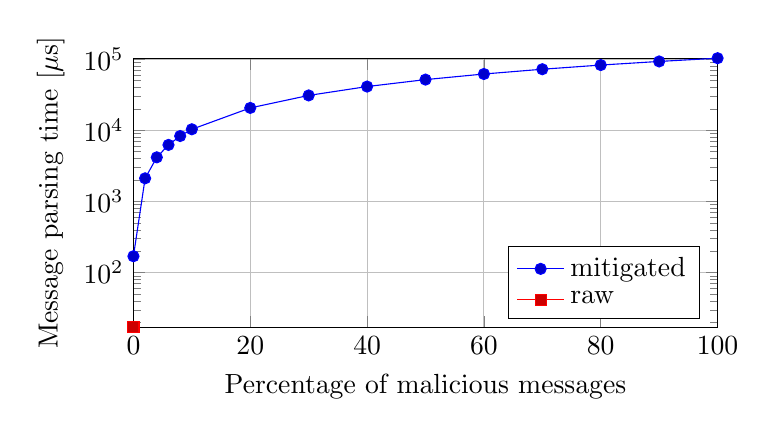
\begin{tikzpicture}
    \begin{semilogyaxis}[
      height=5cm, 
      width=9cm, 
      grid=major, 
      xlabel={Percentage of malicious messages}, 
      ylabel={Message parsing time [$\mu$s]},
      xmin=0,xmax=100,
      ymin=17,ymax=103326,
      legend pos=south east,
      legend cell align={left}
      ]

      \addplot coordinates {
        (0,170)
        (2,2116)
        (4,4177)
        (6,6245)
        (8,8324)
        (10,10353)
        (20,20672)
        (30,30974)
        (40,41276)
        (50,51680)
        (60,61965)
        (70,72318)
        (80,82756)
        (90,93058)
        (100,103326)
      };
      \addlegendentry{mitigated}

      \addplot coordinates {
        (0, 17)
      };
      \addlegendentry{raw}
    \end{semilogyaxis}
  \end{tikzpicture}
\end{figure}

Another attack is one that sends messages to the system that are just under the \pcode{maximum-size} limit. With sufficient, though still fairly low number of messages, this will cause the system to fail with out-of-memory error; and this cannot be contained in a separate thread pool; a proof-of-concept code is shown in \autoref{code:malicious-message-pb-oom}.

\begin{lstlisting}[caption={Malicious message}, label={code:malicious-message-pb-oom}, language=Scala, escapechar=|]
|Construct a malicious message that specifies the $greeting$ property to be a string of $10485759$ characters. The eager parser makes a copy of the entire buffer, the streaming parser reads \& allocates the memory by chunks.|
val b  = Array[Byte](8, 1, 18, -1, -1, -1, 4)
val mb = Array.fill(b.length + 10485759)(65.toByte)
Array.copy(b, 0, mb, 0, b.length)

|Simulate in flight processing, even though we count to 200 the OOM happens around 165|
val inFlight: ArrayBuffer[X] = ArrayBuffer()
for (_ <- 0 to 200) {
  val x = X.parseFrom(mb)
  |$\uparrow$|
  |Exception in thread "main" java.lang.OutOfMemoryError:\P |
  |  Java heap space|
  |  at \ldots StringCoding.decode(\ldots:215)|
  |  at \ldots String.\textless{}init\textgreater(\ldots:463)|
  |  at \ldots ArrayDecoder.readString(\ldots 773)|
  |  \ldots|
  inFlight += x
}
\end{lstlisting}

It is particularly dangerous if the system is designed to read messages from a journal in a transactional-like manner: because the message causes a crash that cannot be handled, the \pcode{read} operation is never confirmed; upon restart, the system will read the malicious message again. While the implementation of the protocol decoding code should be as robust as possible, it is necessary to consider other mechanisms to skip a message that causes fatal errors. A useful testing approach is to provide a generator that can yield malicious payloads for any message type; see \autoref{code:pb-generator-malicious}.

\begin{lstlisting}[caption={Malicious Generator}, label={code:pb-generator-malicious}, language=Scala, escapechar=|]
object MessageGenerator {
  |Constructs a \emph{malicious} generator for a type of type $A$,|
  |with optionally provided hints for the fields|
  def msgM[A <: GeneratedMessage with Message[A]]
      (implicit cmp: GeneratedMessageCompanion[A], 
       hint: Hint[A] = noHint): Gen[A] = ...
}
\end{lstlisting}

\subsection{Practical application}
In the first application of the chaos approaches \& tooling we found three distinct classes of problems: the deserialization code, the tracing and logging code, and the error recovery and retry code. Once discovered, all were simple to fix, but the consequence of missing the bugs would have resulted in complete loss of service had similar messages reached our system in production.

The mitigation for first class of issues focused on setting strict message size limits, and wrapping the decoding code in a separate thread pool, which provided the necessary isolation. The next issue found was in the logging machinery: too-deeply-nested messages resulted in the failures in the structured logging code. Both issues cause the services to react in the same way, the system as a whole didn't crash because it is using Akka supervision, instead individual services or actors crashed consuming a given message from Kafka either due to the deserializer or the logger, the message processing wasn't acknowledged. After restart the services consumed the same last batch of acknowledged messages creating an endless loop of restarts, meaning the messages before the malicious one are reprocessed and no messages after the culprit can be consumed. 

\printbibliography

\end{document}
